\documentclass[tikz,border=30pt]{standalone}
\usepackage{amsmath,amssymb}
\usetikzlibrary{calc}

\begin{document}
	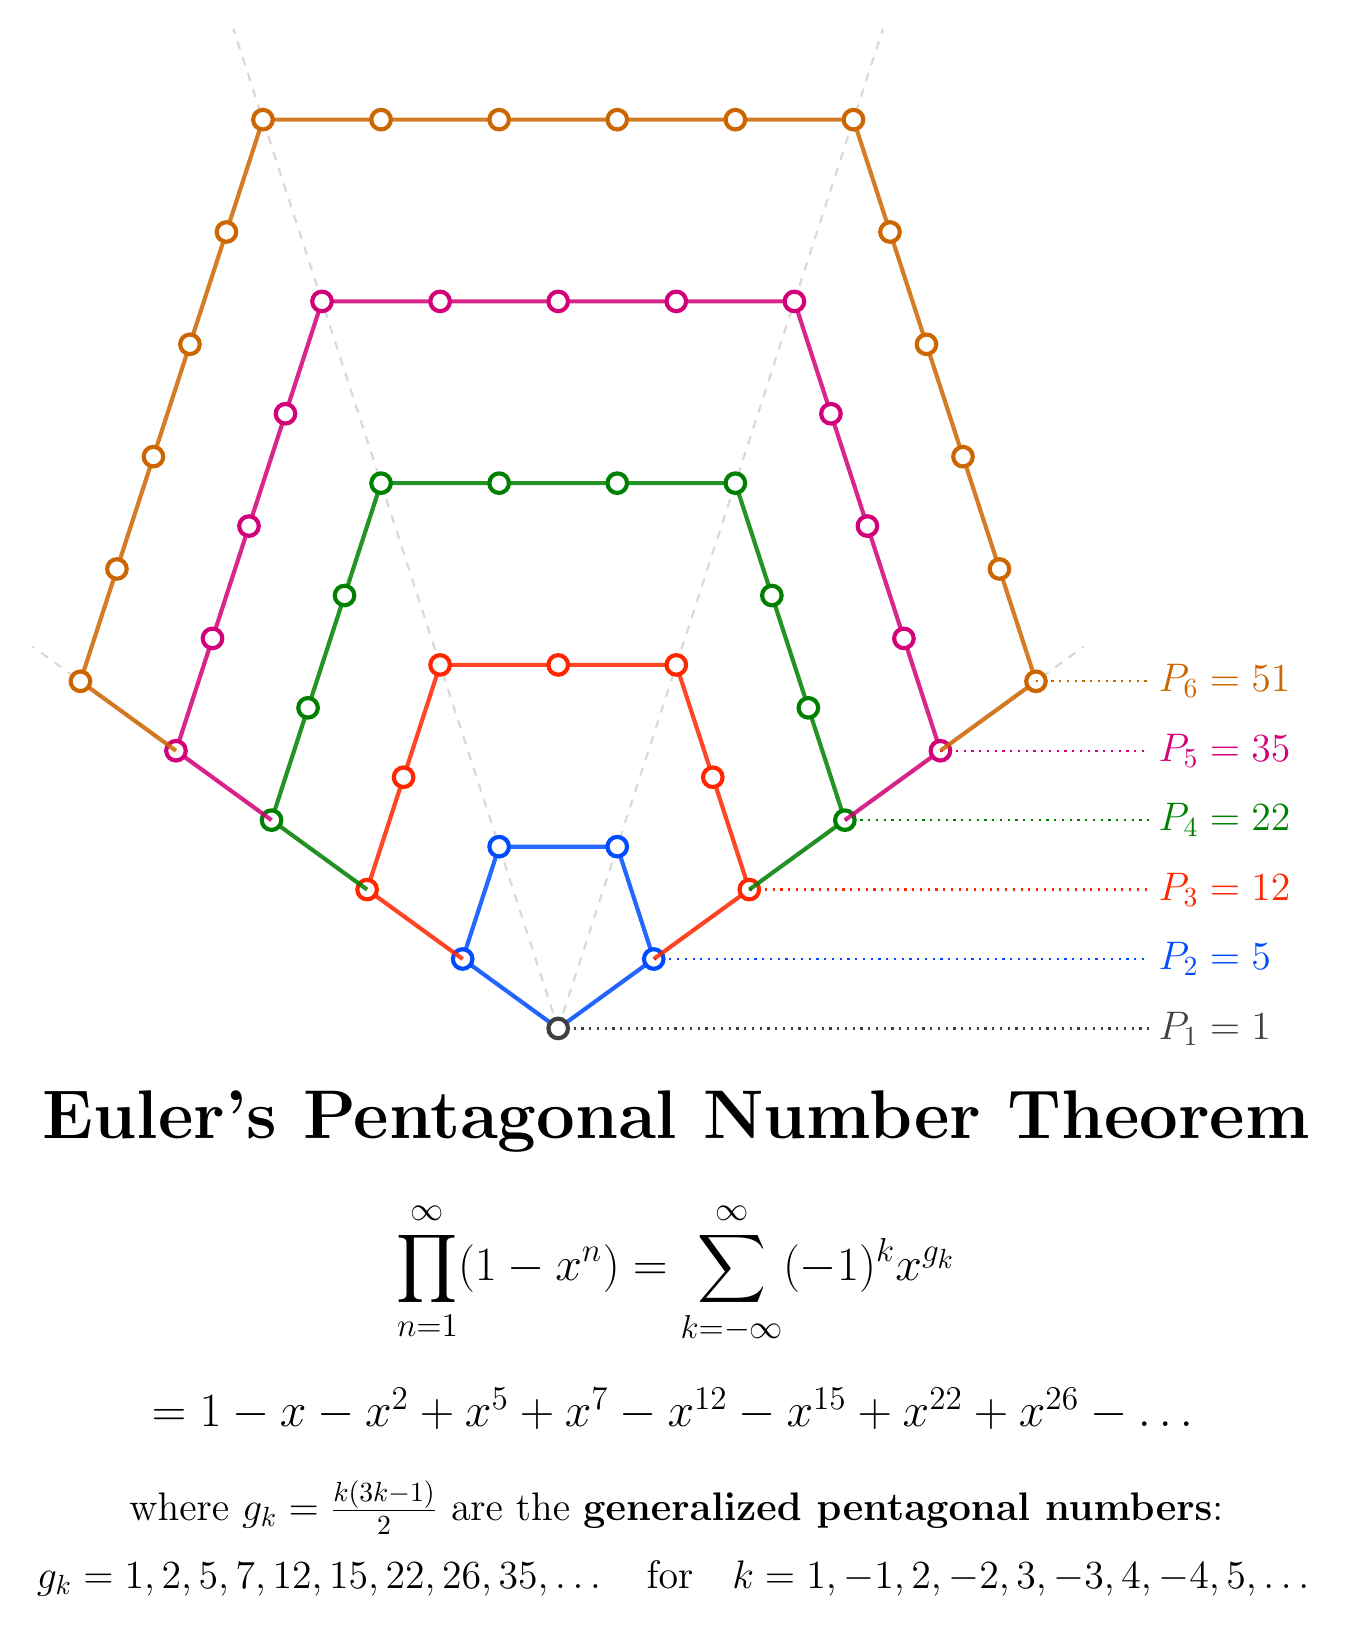
\begin{tikzpicture}[
		dot/.style={circle, fill=white, draw=#1, line width=1.5pt, inner sep=2.5pt},
		edge/.style={line width=1.5pt, draw=#1, opacity=0.85}
		]
		
		% ==========================================
		% COLOR PALETTE FOR LAYERS
		% ==========================================
		\colorlet{col1}{black!75}
		\colorlet{col2}{blue!70!cyan}
		\colorlet{col3}{red!70!orange}
		\colorlet{col4}{green!50!black}
		\colorlet{col5}{purple!70!magenta}
		\colorlet{col6}{orange!80!black}
		
		% Define the maximum number of layers
		\def\maxN{6}
		
		% ==========================================
		% INVISIBLE VERTEX CALCULATION FOR RAYS
		% ==========================================
		% We calculate the outer layer strictly to draw the background guide rays
		\pgfmathtruncatemacro{\maxS}{\maxN-1}
		\coordinate (MaxV1) at ({\maxS*1.5*cos(36)}, {\maxS*1.5*sin(36)});
		\coordinate (MaxV2) at ($(MaxV1) + ({\maxS*1.5*cos(108)}, {\maxS*1.5*sin(108)})$);
		\coordinate (MaxV3) at ($(MaxV2) + ({-1.5*\maxS}, 0)$);
		\coordinate (MaxV4) at ({-1.5*\maxS*cos(36)}, {1.5*\maxS*sin(36)});
		
		% Draw background structural rays passing through the vertices
		\foreach \V in {MaxV1, MaxV2, MaxV3, MaxV4} {
			\draw[thick, gray!30, dashed] (0,0) -- ($(0,0)!1.1!(\V)$);
		}
		
		% ==========================================
		% ORIGIN (n=1, P_1=1)
		% ==========================================
		\coordinate (P_0) at (0,0);
		
		% Label for origin
		\draw[dotted, col1, thick] (P_0) -- (7.5, 0);
		\node[right, font=\bfseries\Large, text=col1] at (7.5, 0) {$P_1 = 1$};
		
		% ==========================================
		% NESTED PENTAGONS (n=2 to 6)
		% ==========================================
		\foreach \n in {2, ..., \maxN} {
			% Using truncatemacro to ensure integers, preventing the anchor "." error
			\pgfmathtruncatemacro{\s}{\n-1}
			\pgfmathtruncatemacro{\prevS}{\s-1}
			\colorlet{ccol}{col\n}
			
			% Calculate vertices for the current layer \s
			\coordinate (V\s-1) at ({\s*1.5*cos(36)}, {\s*1.5*sin(36)});
			\coordinate (V\s-2) at ($(V\s-1) + ({\s*1.5*cos(108)}, {\s*1.5*sin(108)})$);
			\coordinate (V\s-3) at ($(V\s-2) + ({-1.5*\s}, 0)$);
			\coordinate (V\s-4) at ({-1.5*\s*cos(36)}, {1.5*\s*sin(36)});
			
			% Draw inner radial edges bridging the previous layer to the new one
			\coordinate (prevV-1) at ({\prevS*1.5*cos(36)}, {\prevS*1.5*sin(36)});
			\coordinate (prevV-4) at ({-\prevS*1.5*cos(36)}, {\prevS*1.5*sin(36)});
			\draw[edge=ccol] (prevV-1) -- (V\s-1);
			\draw[edge=ccol] (prevV-4) -- (V\s-4);
			
			% Draw the 3 outer perimeter edges of the pentagon
			\draw[edge=ccol] (V\s-1) -- (V\s-2) -- (V\s-3) -- (V\s-4);
			
			% Distribute dots evenly along the edges to mathematically match P_n
			% Edge 1: V1 to V2
			\foreach \k in {0,...,\s} {
				\pgfmathsetmacro{\mypos}{\k/\s} % Replaced \frac with \mypos
				\coordinate (D) at ($(V\s-1)!\mypos!(V\s-2)$);
				\node[dot=ccol] at (D) {};
			}
			% Edge 2: V2 to V3 (skip k=0 to avoid overlapping corners)
			\foreach \k in {1,...,\s} {
				\pgfmathsetmacro{\mypos}{\k/\s}
				\coordinate (D) at ($(V\s-2)!\mypos!(V\s-3)$);
				\node[dot=ccol] at (D) {};
			}
			% Edge 3: V3 to V4 (skip k=0)
			\foreach \k in {1,...,\s} {
				\pgfmathsetmacro{\mypos}{\k/\s}
				\coordinate (D) at ($(V\s-3)!\mypos!(V\s-4)$);
				\node[dot=ccol] at (D) {};
			}
			
			% Cumulative Pentagonal Number formula: P_n = n(3n-1)/2
			\pgfmathtruncatemacro{\Pn}{\n*(3*\n-1)/2}
			
			% Dotted guides and Labels on the right side
			\draw[dotted, ccol, thick] (V\s-1) -- (7.5, {\s*1.5*sin(36)});
			\node[right, font=\bfseries\Large, text=ccol] at (7.5, {\s*1.5*sin(36)}) {$P_{\n} = \Pn$};
		}
		
		% Draw the central origin dot last so it overlaps cleanly
		\node[dot=col1] at (P_0) {};
		
		% ==========================================
		% EULER'S THEOREM FORMULA & EXPLANATION
		% ==========================================
		\node[align=center] at (1.5, -4) {
			{\Huge \textbf{Euler's Pentagonal Number Theorem}} \\[6mm]
			{\LARGE $\displaystyle \prod_{n=1}^\infty (1-x^n) = \sum_{k=-\infty}^\infty (-1)^k x^{g_k}$} \\[5mm]
			{\LARGE $= 1 - x - x^2 + x^5 + x^7 - x^{12} - x^{15} + x^{22} + x^{26} - \dots$} \\[6mm]
			{\Large where $g_k = \frac{k(3k-1)}{2}$ are the \textbf{generalized pentagonal numbers}:} \\[3mm]
			{\Large $g_k = 1, 2, 5, 7, 12, 15, 22, 26, 35, \dots \quad \text{for} \quad k = 1, -1, 2, -2, 3, -3, 4, -4, 5, \dots$}
		};
		
	\end{tikzpicture}
\end{document}